% Options for packages loaded elsewhere
\PassOptionsToPackage{unicode}{hyperref}
\PassOptionsToPackage{hyphens}{url}
%
\documentclass[
  ignorenonframetext,
]{beamer}
\usepackage{pgfpages}
\setbeamertemplate{caption}[numbered]
\setbeamertemplate{caption label separator}{: }
\setbeamercolor{caption name}{fg=normal text.fg}
\beamertemplatenavigationsymbolsempty
% Prevent slide breaks in the middle of a paragraph
\widowpenalties 1 10000
\raggedbottom
\setbeamertemplate{part page}{
  \centering
  \begin{beamercolorbox}[sep=16pt,center]{part title}
    \usebeamerfont{part title}\insertpart\par
  \end{beamercolorbox}
}
\setbeamertemplate{section page}{
  \centering
  \begin{beamercolorbox}[sep=12pt,center]{part title}
    \usebeamerfont{section title}\insertsection\par
  \end{beamercolorbox}
}
\setbeamertemplate{subsection page}{
  \centering
  \begin{beamercolorbox}[sep=8pt,center]{part title}
    \usebeamerfont{subsection title}\insertsubsection\par
  \end{beamercolorbox}
}
\AtBeginPart{
  \frame{\partpage}
}
\AtBeginSection{
  \ifbibliography
  \else
    \frame{\sectionpage}
  \fi
}
\AtBeginSubsection{
  \frame{\subsectionpage}
}
\usepackage{amsmath,amssymb}
\usepackage{iftex}
\ifPDFTeX
  \usepackage[T1]{fontenc}
  \usepackage[utf8]{inputenc}
  \usepackage{textcomp} % provide euro and other symbols
\else % if luatex or xetex
  \usepackage{unicode-math} % this also loads fontspec
  \defaultfontfeatures{Scale=MatchLowercase}
  \defaultfontfeatures[\rmfamily]{Ligatures=TeX,Scale=1}
\fi
\usepackage{lmodern}
\ifPDFTeX\else
  % xetex/luatex font selection
\fi
% Use upquote if available, for straight quotes in verbatim environments
\IfFileExists{upquote.sty}{\usepackage{upquote}}{}
\IfFileExists{microtype.sty}{% use microtype if available
  \usepackage[]{microtype}
  \UseMicrotypeSet[protrusion]{basicmath} % disable protrusion for tt fonts
}{}
\makeatletter
\@ifundefined{KOMAClassName}{% if non-KOMA class
  \IfFileExists{parskip.sty}{%
    \usepackage{parskip}
  }{% else
    \setlength{\parindent}{0pt}
    \setlength{\parskip}{6pt plus 2pt minus 1pt}}
}{% if KOMA class
  \KOMAoptions{parskip=half}}
\makeatother
\usepackage{xcolor}
\newif\ifbibliography
\usepackage{graphicx}
\makeatletter
\def\maxwidth{\ifdim\Gin@nat@width>\linewidth\linewidth\else\Gin@nat@width\fi}
\def\maxheight{\ifdim\Gin@nat@height>\textheight\textheight\else\Gin@nat@height\fi}
\makeatother
% Scale images if necessary, so that they will not overflow the page
% margins by default, and it is still possible to overwrite the defaults
% using explicit options in \includegraphics[width, height, ...]{../figures/}
\setkeys{Gin}{width=\maxwidth,height=\maxheight,keepaspectratio}
% Set default figure placement to htbp
\makeatletter
\def\fps@figure{htbp}
\makeatother
\setlength{\emergencystretch}{3em} % prevent overfull lines
\providecommand{\tightlist}{%
  \setlength{\itemsep}{0pt}\setlength{\parskip}{0pt}}
\setcounter{secnumdepth}{-\maxdimen} % remove section numbering
% Slide layout defaults for warning-clean scientific decks.
\usepackage{etoolbox}
\IfFileExists{xurl.sty}{\usepackage{xurl}}{}
\IfFileExists{seqsplit.sty}{\usepackage{seqsplit}}{\newcommand{\seqsplit}[1]{#1}}
\protected\def\breakseq#1{\seqsplit{#1}}
\protected\def\breaktt#1{\begingroup\ttfamily\seqsplit{#1}\endgroup}
\setlength{\emergencystretch}{6em}
\tolerance=5000
\hbadness=10000
\hfuzz=1pt
\setlength{\tabcolsep}{2pt}
\AtBeginEnvironment{longtable}{\tiny\renewcommand{\arraystretch}{0.86}\setlength{\tabcolsep}{1pt}}
\AtBeginEnvironment{tabular}{\tiny\renewcommand{\arraystretch}{0.86}\setlength{\tabcolsep}{1pt}}

% Natbib and cross-reference fallbacks — slides don't load natbib
% or cleveref, but combined-PDF manuscript prose may emit these
% commands. The fallback renders citations as a bracketed key list
% and cross-references as detokenized labels so slides don't fail on
% undefined control sequences or raw underscores. \providecommand is
% a no-op if packages load later.
\providecommand{\citep}[1]{[#1]}
\providecommand{\citet}[1]{#1}
\providecommand{\citealp}[1]{#1}
\providecommand{\citeauthor}[1]{#1}
\providecommand{\citeyear}[1]{#1}
\providecommand{\cref}[1]{\texttt{\detokenize{#1}}}
\providecommand{\Cref}[1]{\texttt{\detokenize{#1}}}

\newtheorem{proposition}{Proposition}
\newtheorem{hypothesis}{Hypothesis}
\ifLuaTeX
  \usepackage{selnolig}  % disable illegal ligatures
\fi
\usepackage{bookmark}
\IfFileExists{xurl.sty}{\usepackage{xurl}}{} % add URL line breaks if available
\urlstyle{same}
\hypersetup{
  hidelinks,
  pdfcreator={LaTeX via pandoc}}

\author{}
\date{}

\begin{document}

\section{Results: Field Overview}\label{results-field-overview}

\begin{frame}[allowframebreaks]{Results: Field Overview}
The de-duplicated corpus for \textbf{\{\{SEARCH\_TERM\_TITLE\}\}}
contains \(N = {{CORPUS_SIZE}}\) records spanning
\{\{YEAR\_START\}\}--\{\{YEAR\_END\}\} (\{\{YEAR\_SPAN\}\} years).
Publication volume grows at a compound annual rate of
\{\{CAGR\_PCT\}\}\% (mean year-over-year growth
\{\{MEAN\_YOY\_GROWTH\_PCT\}\}\%, doubling time \{\{DOUBLING\_TIME\}\}
years), peaking in \{\{PEAK\_YEAR\}\} with \{\{PEAK\_YEAR\_PUBS\}\}
records that year. The growth curve is a first-order descriptive summary
of the retained corpus; it is not a field-wide estimate of research
activity.

\begin{figure}
\centering
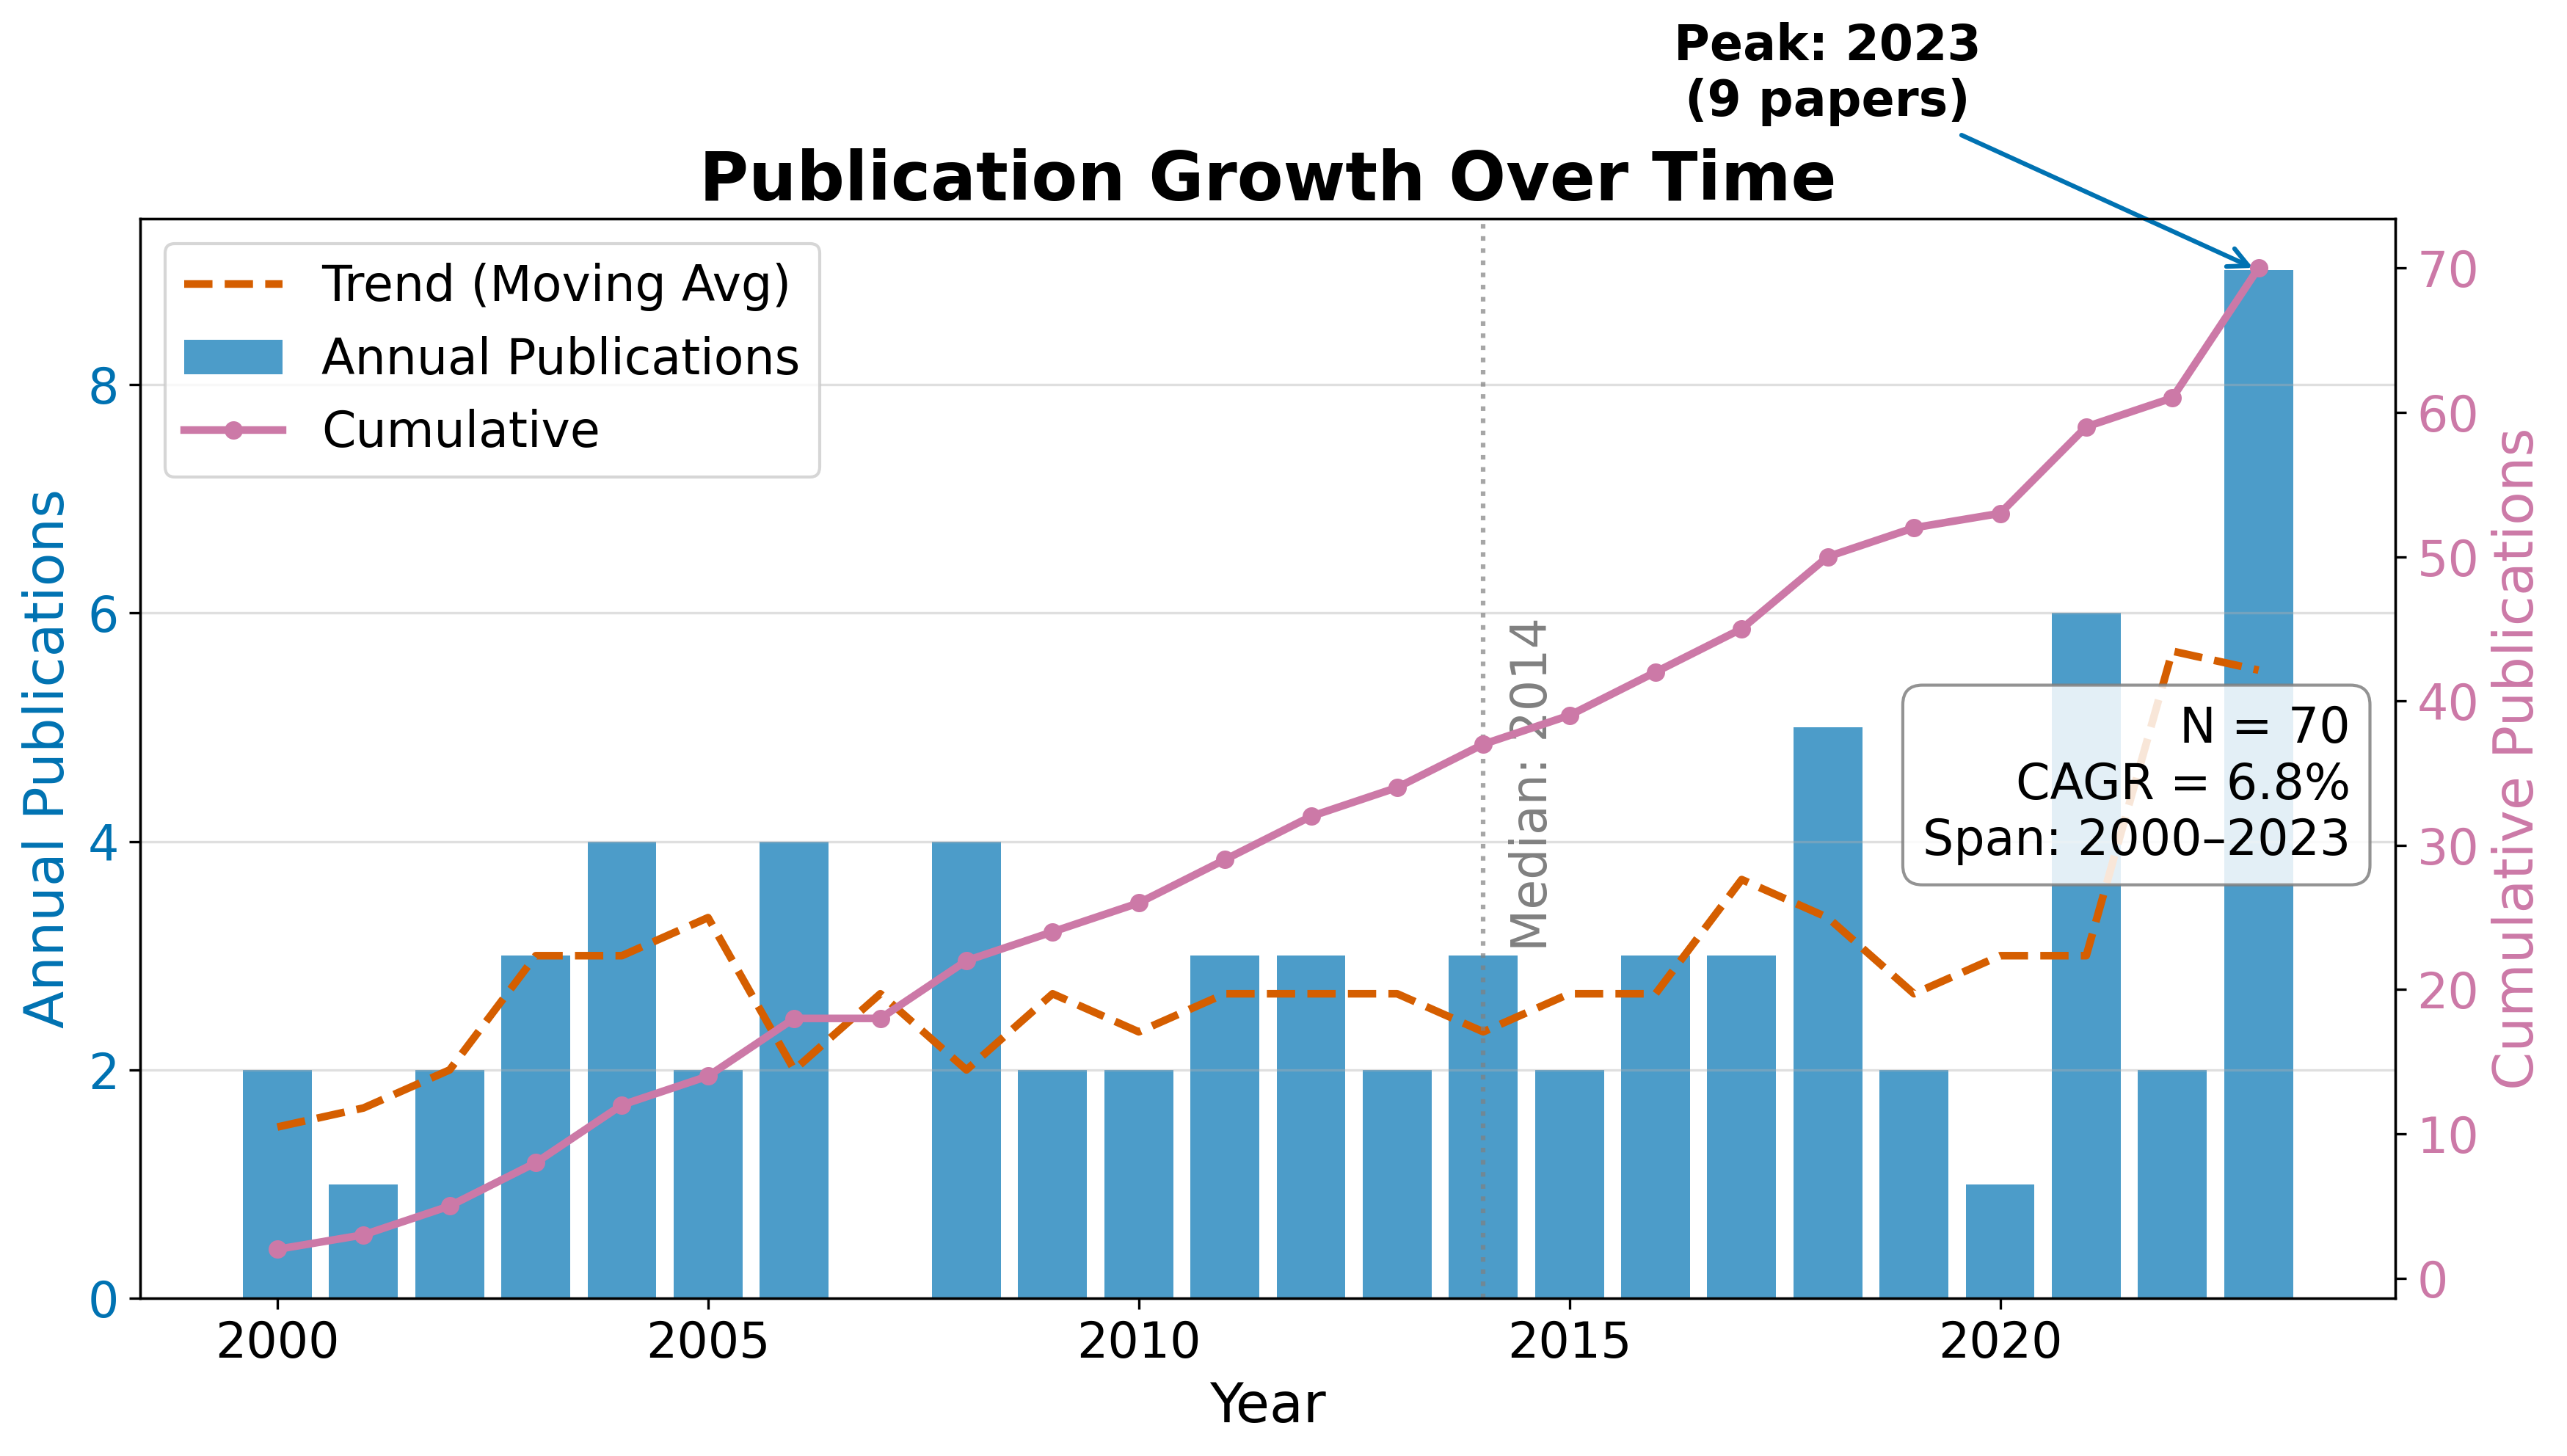
\includegraphics{../figures/growth_curve.png}
\caption{Publication growth curve for \{\{SEARCH\_TERM\_TITLE\}\}.
Annual publication counts (bars) and cumulative total (line) show
sustained growth from \{\{YEAR\_START\}\} through \{\{YEAR\_END\}\},
peaking in \{\{PEAK\_YEAR\}\}.}\label{fig:growth_curve}
\end{figure}
\end{frame}

\begin{frame}[allowframebreaks]{RQ1: Field Size and Growth}
\phantomsection\label{rq1-field-size-and-growth}
The temporal analysis describes a retained literature slice spanning
\{\{YEAR\_SPAN\}\} years. The compound annual growth rate of
\{\{CAGR\_PCT\}\}\% implies a corpus doubling time of approximately
\{\{DOUBLING\_TIME\}\} years under the configured retrieval and indexing
conditions. The peak year \{\{PEAK\_YEAR\}\} contains
\{\{PEAK\_YEAR\_PUBS\}\} retained records; that count may reflect both
publication activity and delays or differences in source indexing, so it
should not be interpreted as a causal trend without a live coverage
audit.

\textbf{Table 1. Top publication years.}

\{\{YEAR\_COUNT\_TABLE\}\}
\end{frame}

\begin{frame}[allowframebreaks]{RQ2: Subfield Composition}
\phantomsection\label{rq2-subfield-composition}
Records distribute across the \{\{N\_SUBFIELDS\}\} configured subfields
as shown in Table 2, with \textbf{\{\{TOP\_SUBFIELD\}\}} the largest
bucket at \{\{TOP\_SUBFIELD\_PCT\}\}\% of the classified corpus. The
dominance of \{\{TOP\_SUBFIELD\}\} is a property of the configured
taxonomy and retained corpus. It is not a domain prevalence estimate
without a live, source-backed review and a documented coverage
assessment.

\textbf{Table 2. Subfield distribution.}

\{\{SUBFIELD\_TABLE\}\}

\begin{figure}
\centering
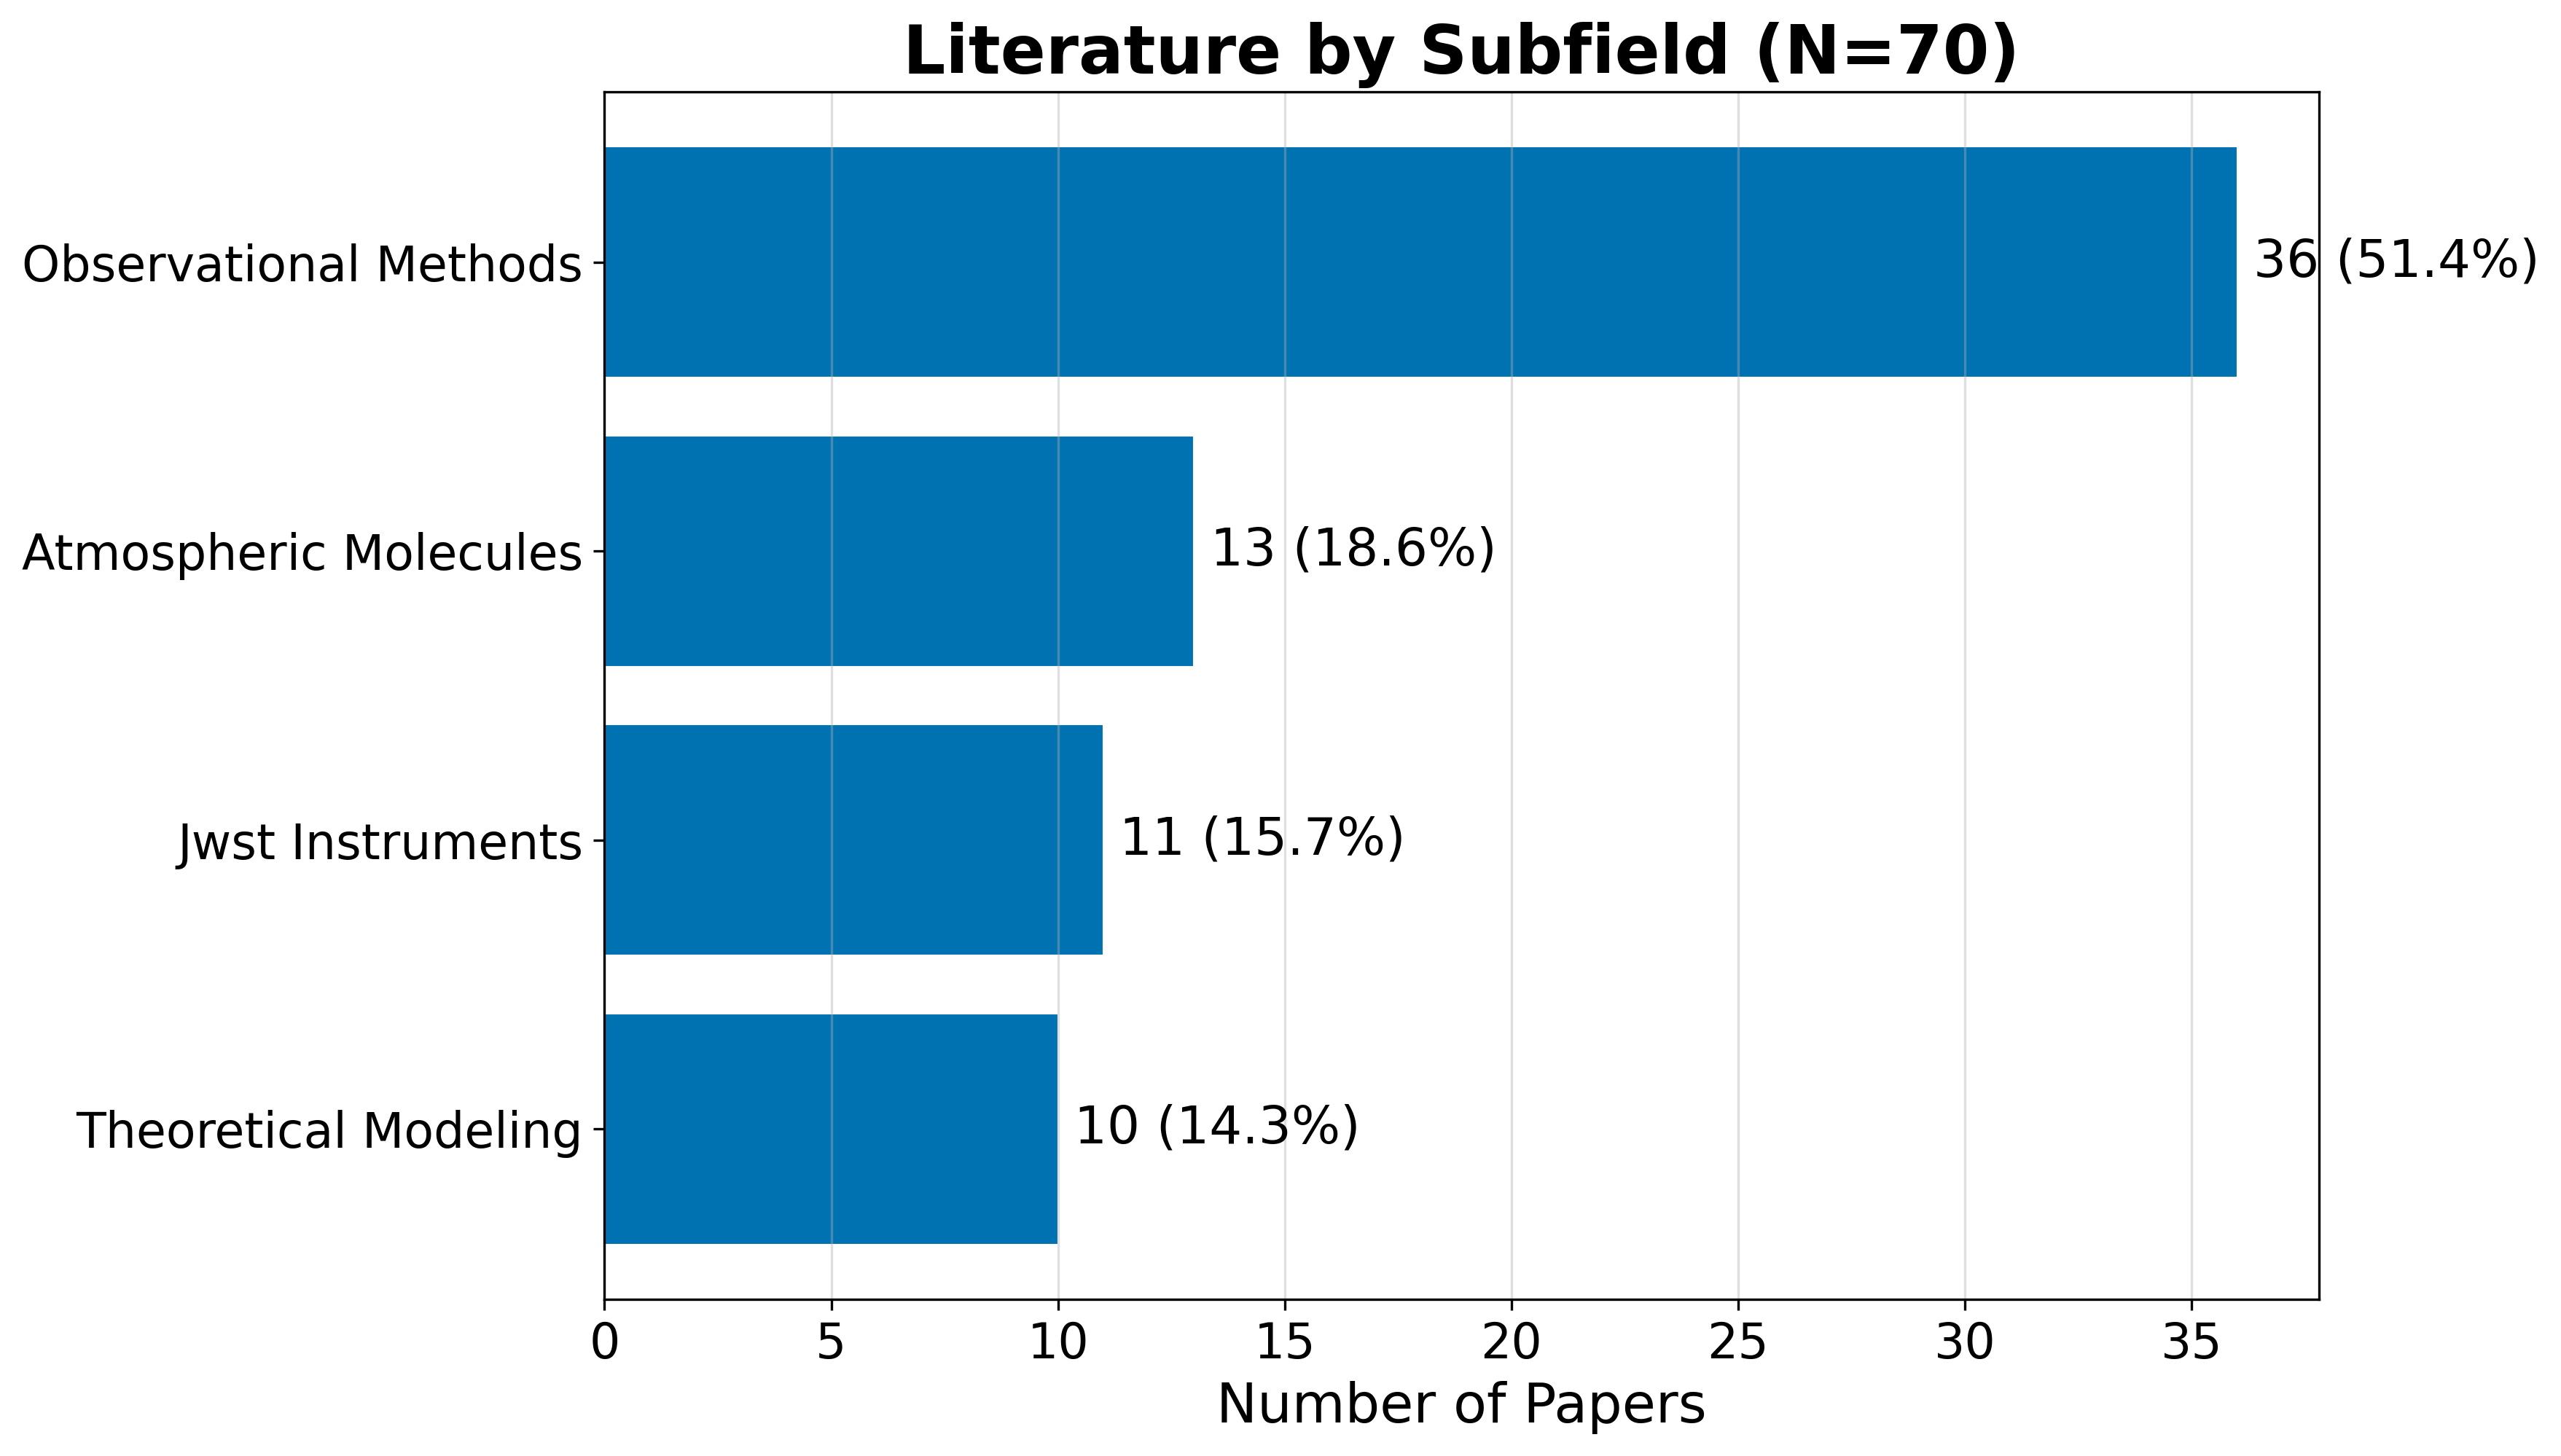
\includegraphics{../figures/field_summary.png}
\caption{Field summary dashboard for \{\{SEARCH\_TERM\_TITLE\}\}. The
dashboard combines corpus size, temporal range, subfield distribution,
and key bibliometric indicators in a single overview
panel.}\label{fig:field_summary}
\end{figure}

\begin{figure}
\centering
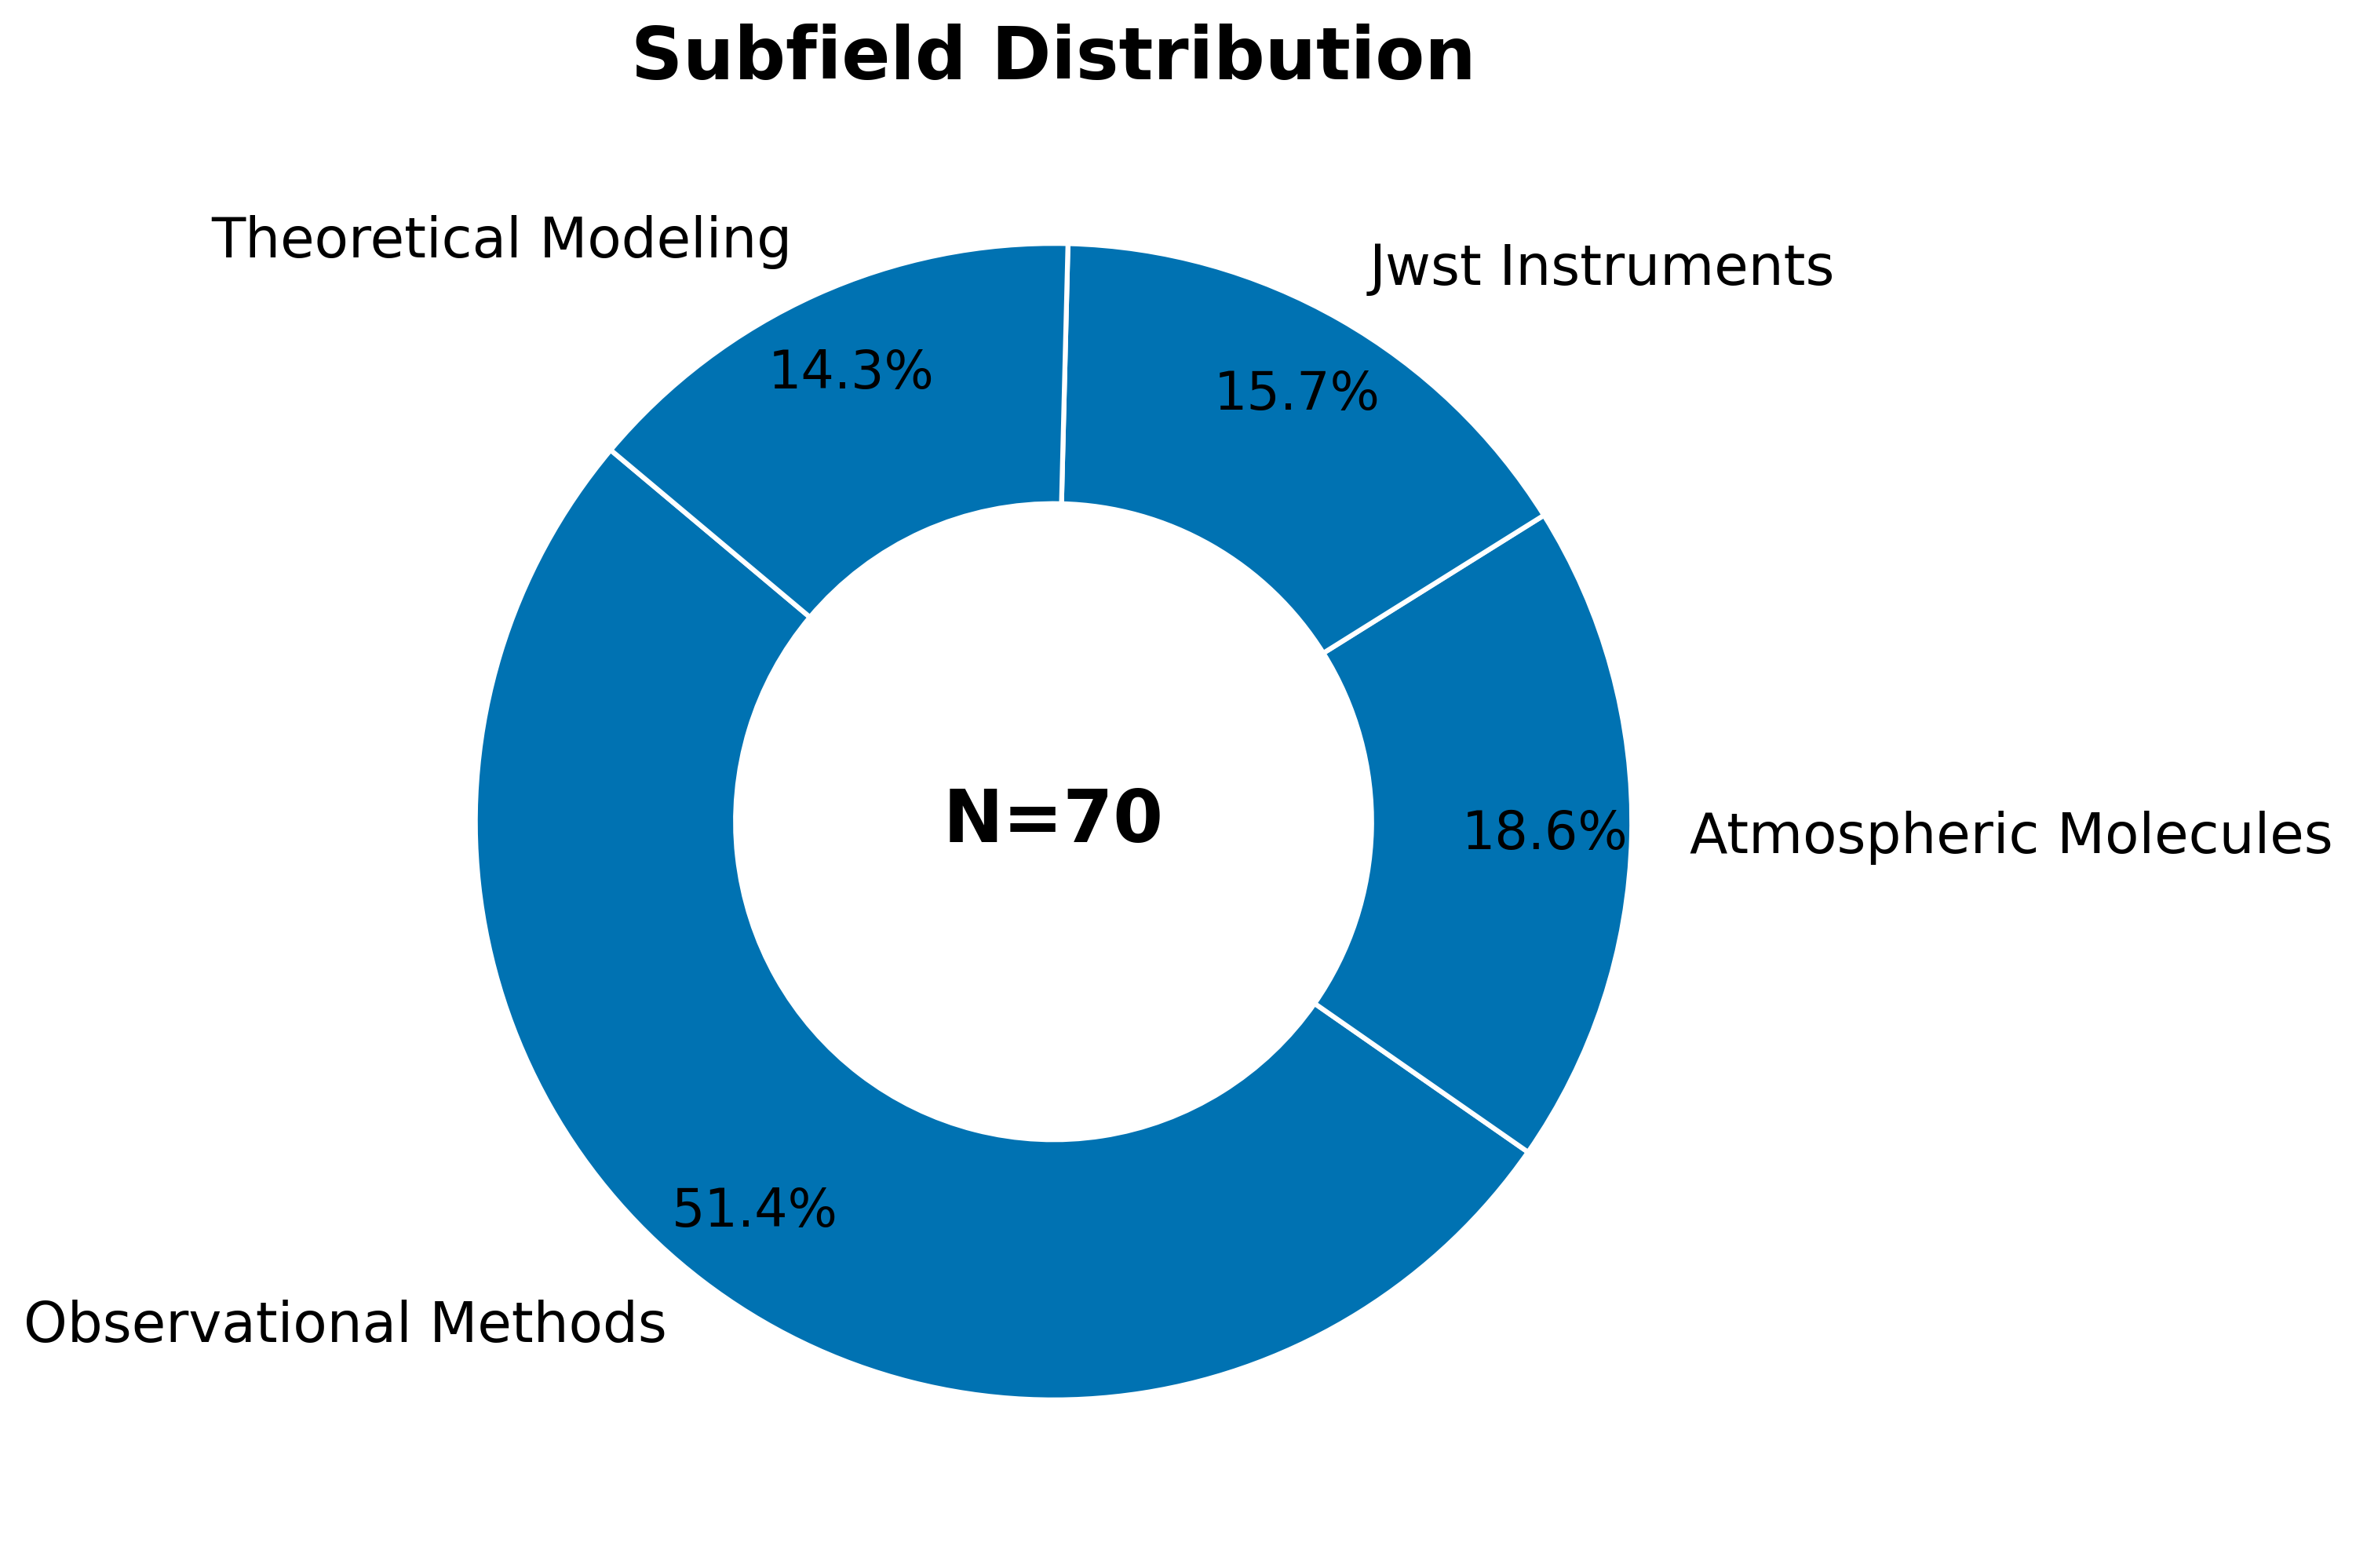
\includegraphics{../figures/subfield_distribution.png}
\caption{Subfield distribution for \{\{SEARCH\_TERM\_TITLE\}\}. The
\{\{N\_SUBFIELDS\}\}-bucket taxonomy shows the relative weight of each
configured sub-area, with \{\{TOP\_SUBFIELD\}\} dominant at
\{\{TOP\_SUBFIELD\_PCT\}\}\%.}\label{fig:subfield_distribution}
\end{figure}

\newpage

\begin{figure}
\centering
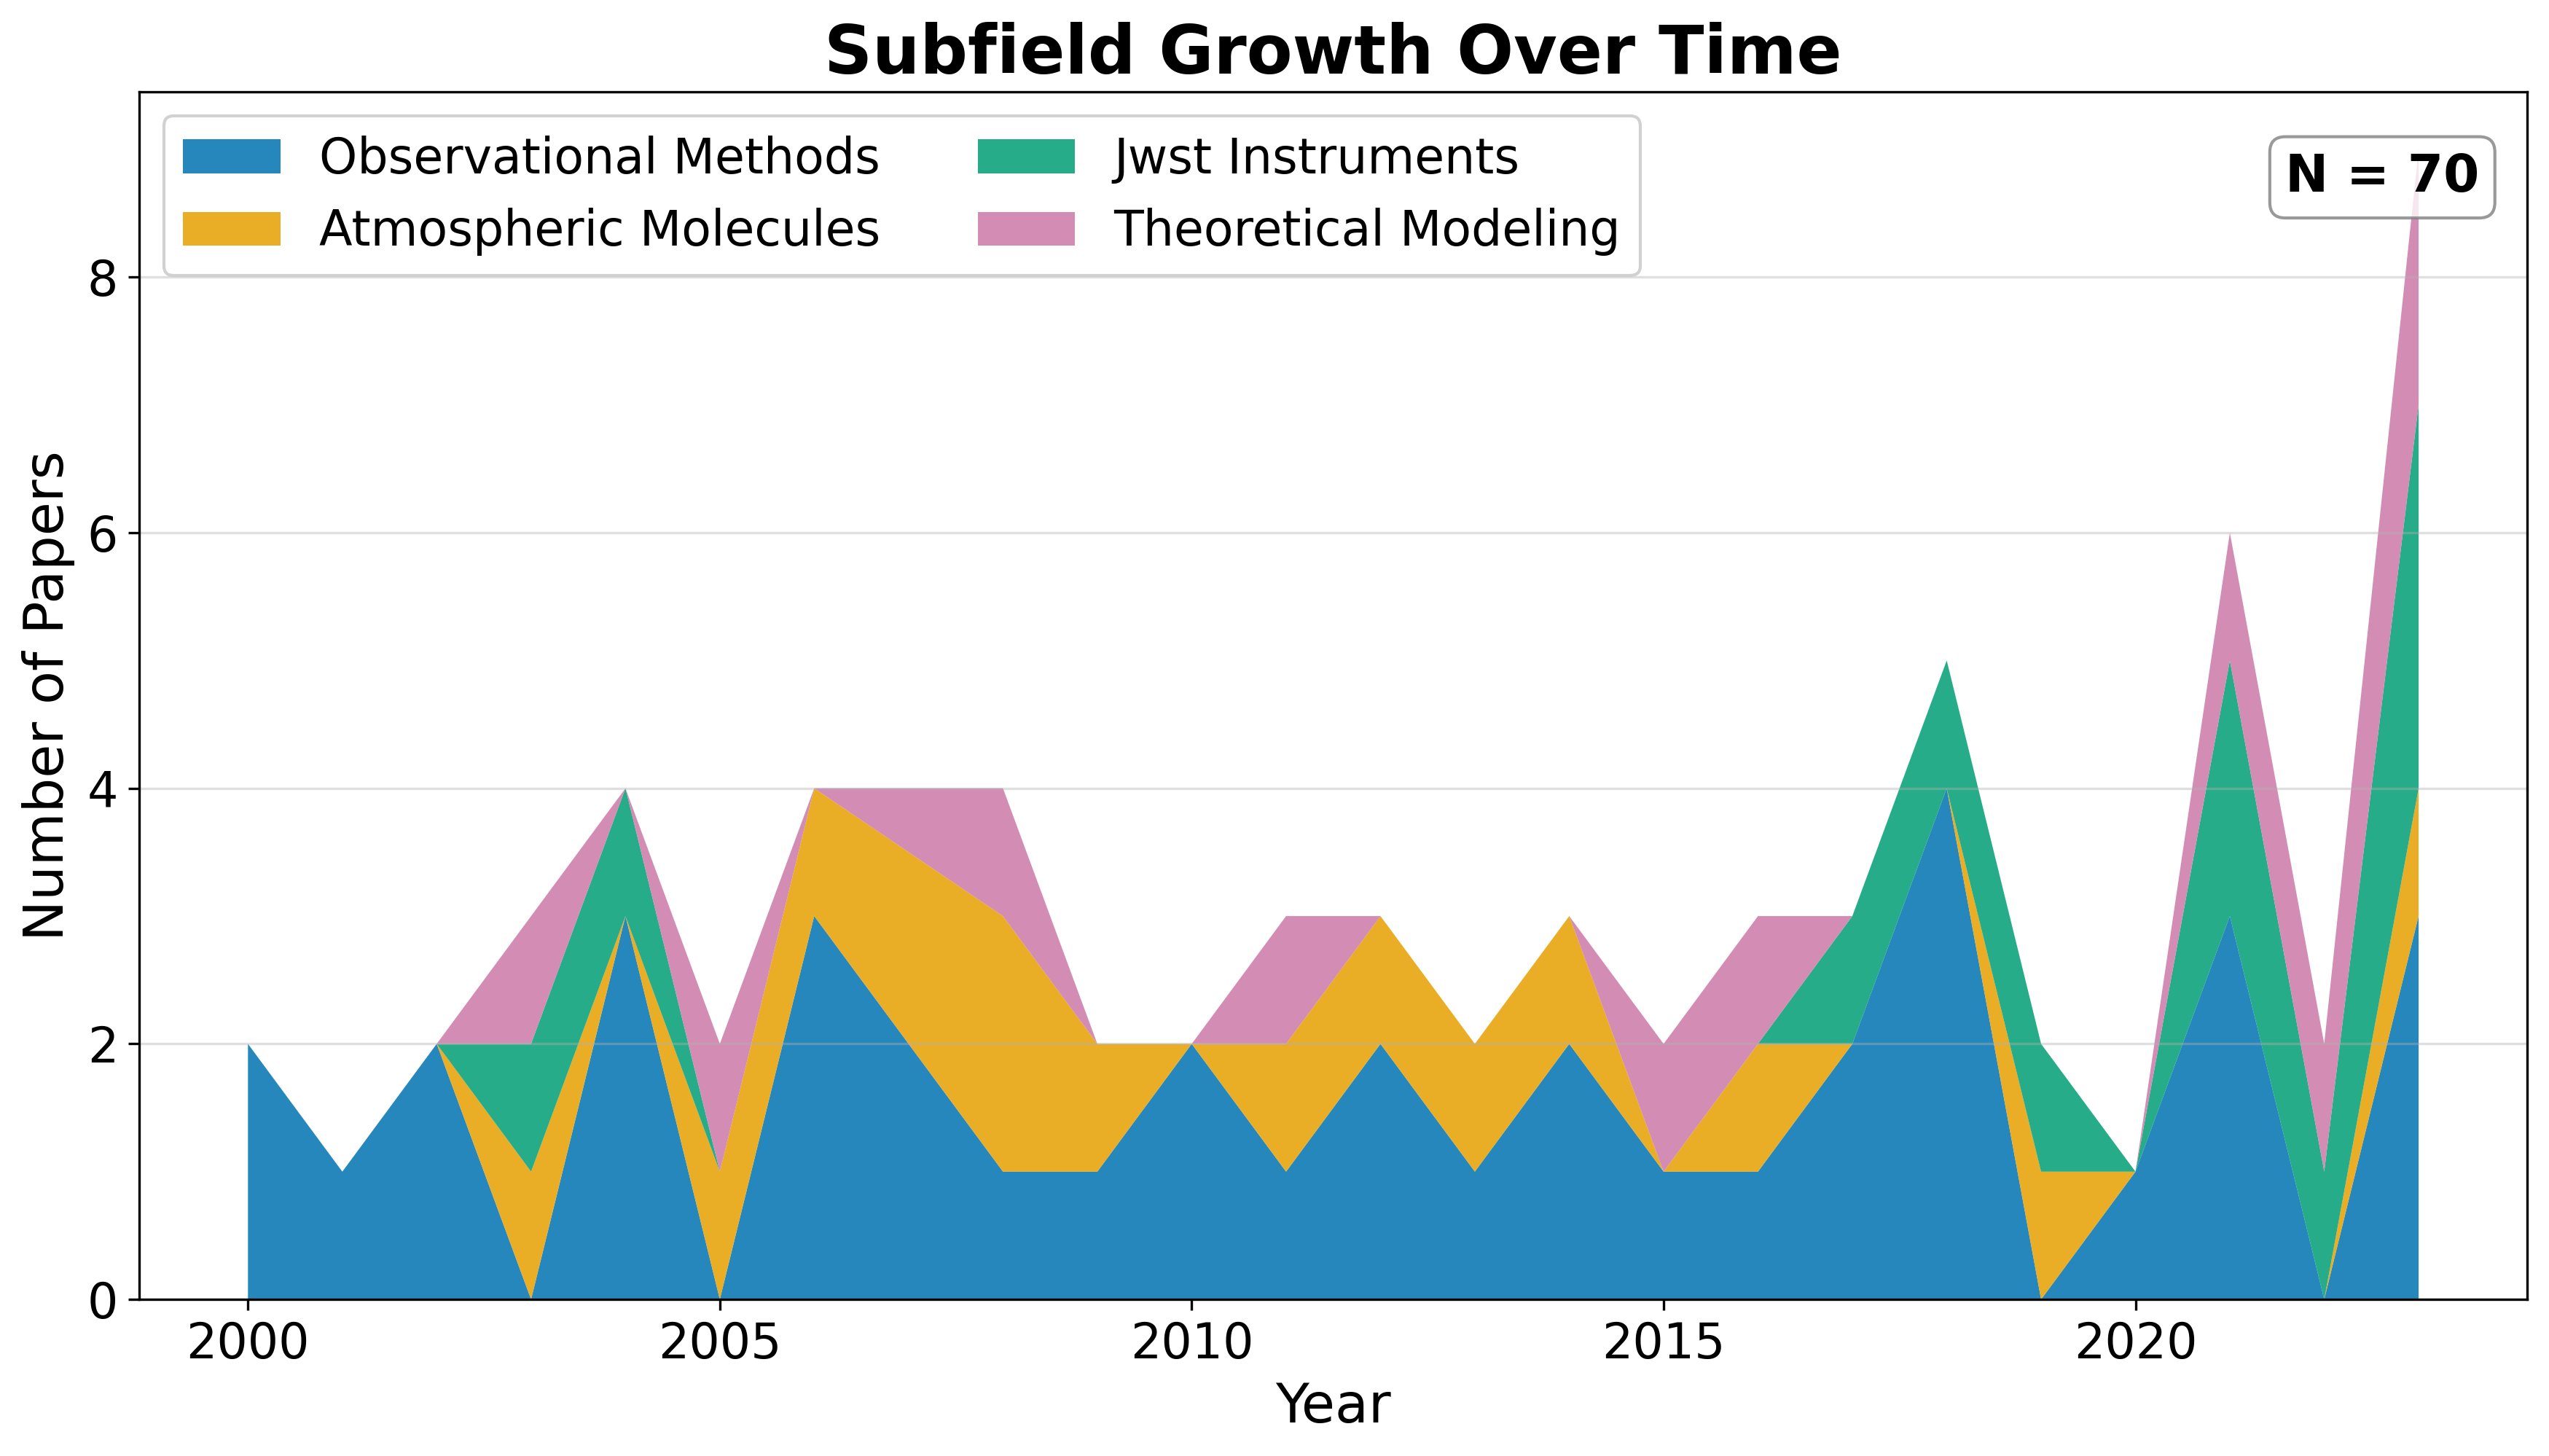
\includegraphics{../figures/subfield_timeline.png}
\caption{Subfield timeline for \{\{SEARCH\_TERM\_TITLE\}\}. Stacked
annual publication counts by subfield show how each sub-area has evolved
over time, revealing emerging and declining research
threads.}\label{fig:subfield_timeline}
\end{figure}
\end{frame}

\begin{frame}[allowframebreaks]{Identifier and Full-Text Coverage}
\phantomsection\label{identifier-and-full-text-coverage}
The corpus has measurable identifier coverage: \{\{DOI\_COUNT\}\} of
\{\{CORPUS\_SIZE\}\} records (\{\{PCT\_WITH\_DOI\}\}\%) carry DOIs,
supporting cross-engine de-duplication. OpenAlex IDs are present for
\{\{OPENALEX\_ID\_COUNT\}\} records. Abstract coverage stands at
\{\{ABSTRACT\_COVERAGE\_PCT\}\}\% (\{\{ABSTRACT\_COUNT\}\} records),
which limits the text analytics to that subset. Open-access status is
confirmed for \{\{OA\_PCT\}\}\% of records, and
\{\{PDF\_AVAIL\_PCT\}\}\% have a direct PDF link.
\end{frame}

\begin{frame}[allowframebreaks]{Descriptive Bibliometrics}
\phantomsection\label{descriptive-bibliometrics}
The corpus spans \{\{UNIQUE\_AUTHORS\}\} unique authors across
\{\{CORPUS\_SIZE\}\} papers, yielding a mean of
\{\{PAPERS\_PER\_AUTHOR\_MEAN\}\} papers per author. Citation counts
range from zero to \{\{CITATION\_MAX\}\} (mean \{\{CITATION\_MEAN\}\},
median \{\{CITATION\_MEDIAN\}\}), with a total of
\{\{CITATION\_TOTAL\}\} citations across the corpus. The Gini
coefficient of citation concentration is \{\{GINI\_COEFFICIENT\}\}. This
statistic describes concentration within the retained corpus and should
not be generalized to citation behavior in the field.

\textbf{Table 3. Citation count distribution.}

\{\{CITATION\_DIST\_TABLE\}\}

\begin{figure}
\centering
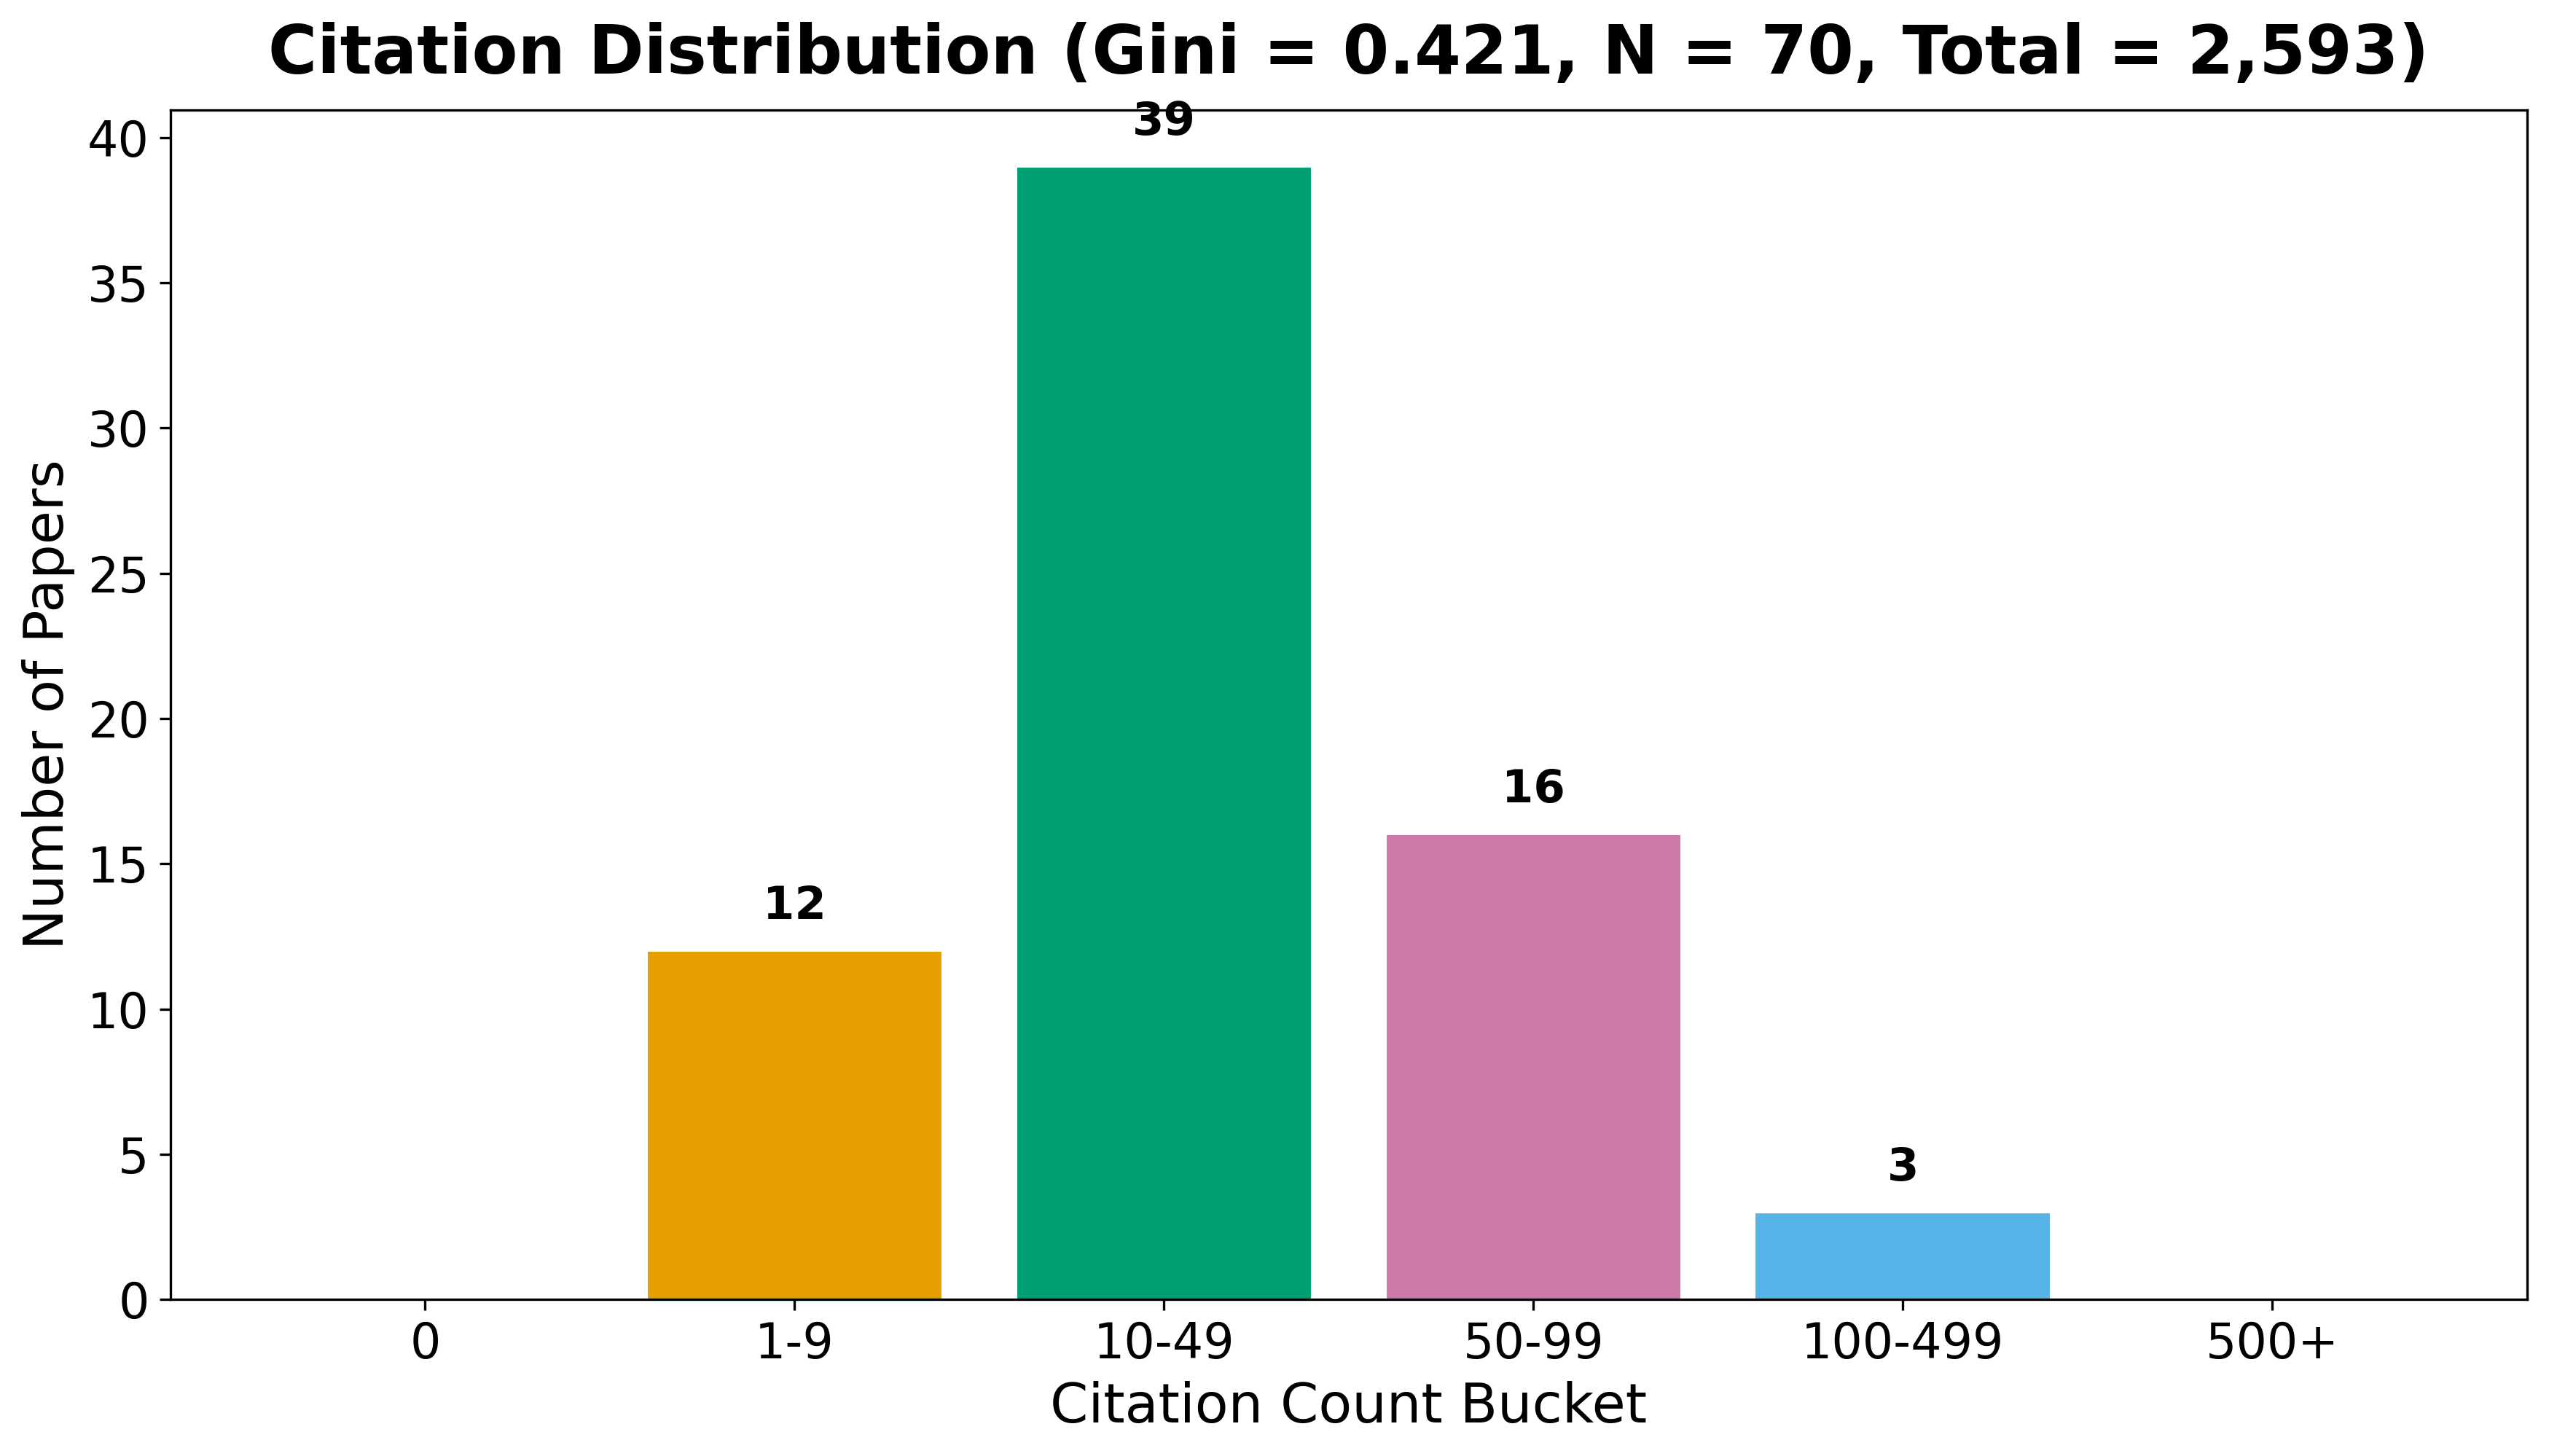
\includegraphics{../figures/citation_distribution.png}
\caption{Citation distribution for \{\{SEARCH\_TERM\_TITLE\}\}. The
histogram shows the number of papers in each citation-count bucket, with
the Gini coefficient annotated. The distribution is a descriptive
property of the retained corpus.}\label{fig:citation_distribution}
\end{figure}

\newpage

\textbf{Table 4. Top publication venues.}

\{\{TOP\_VENUES\_TABLE\}\}

\begin{figure}
\centering
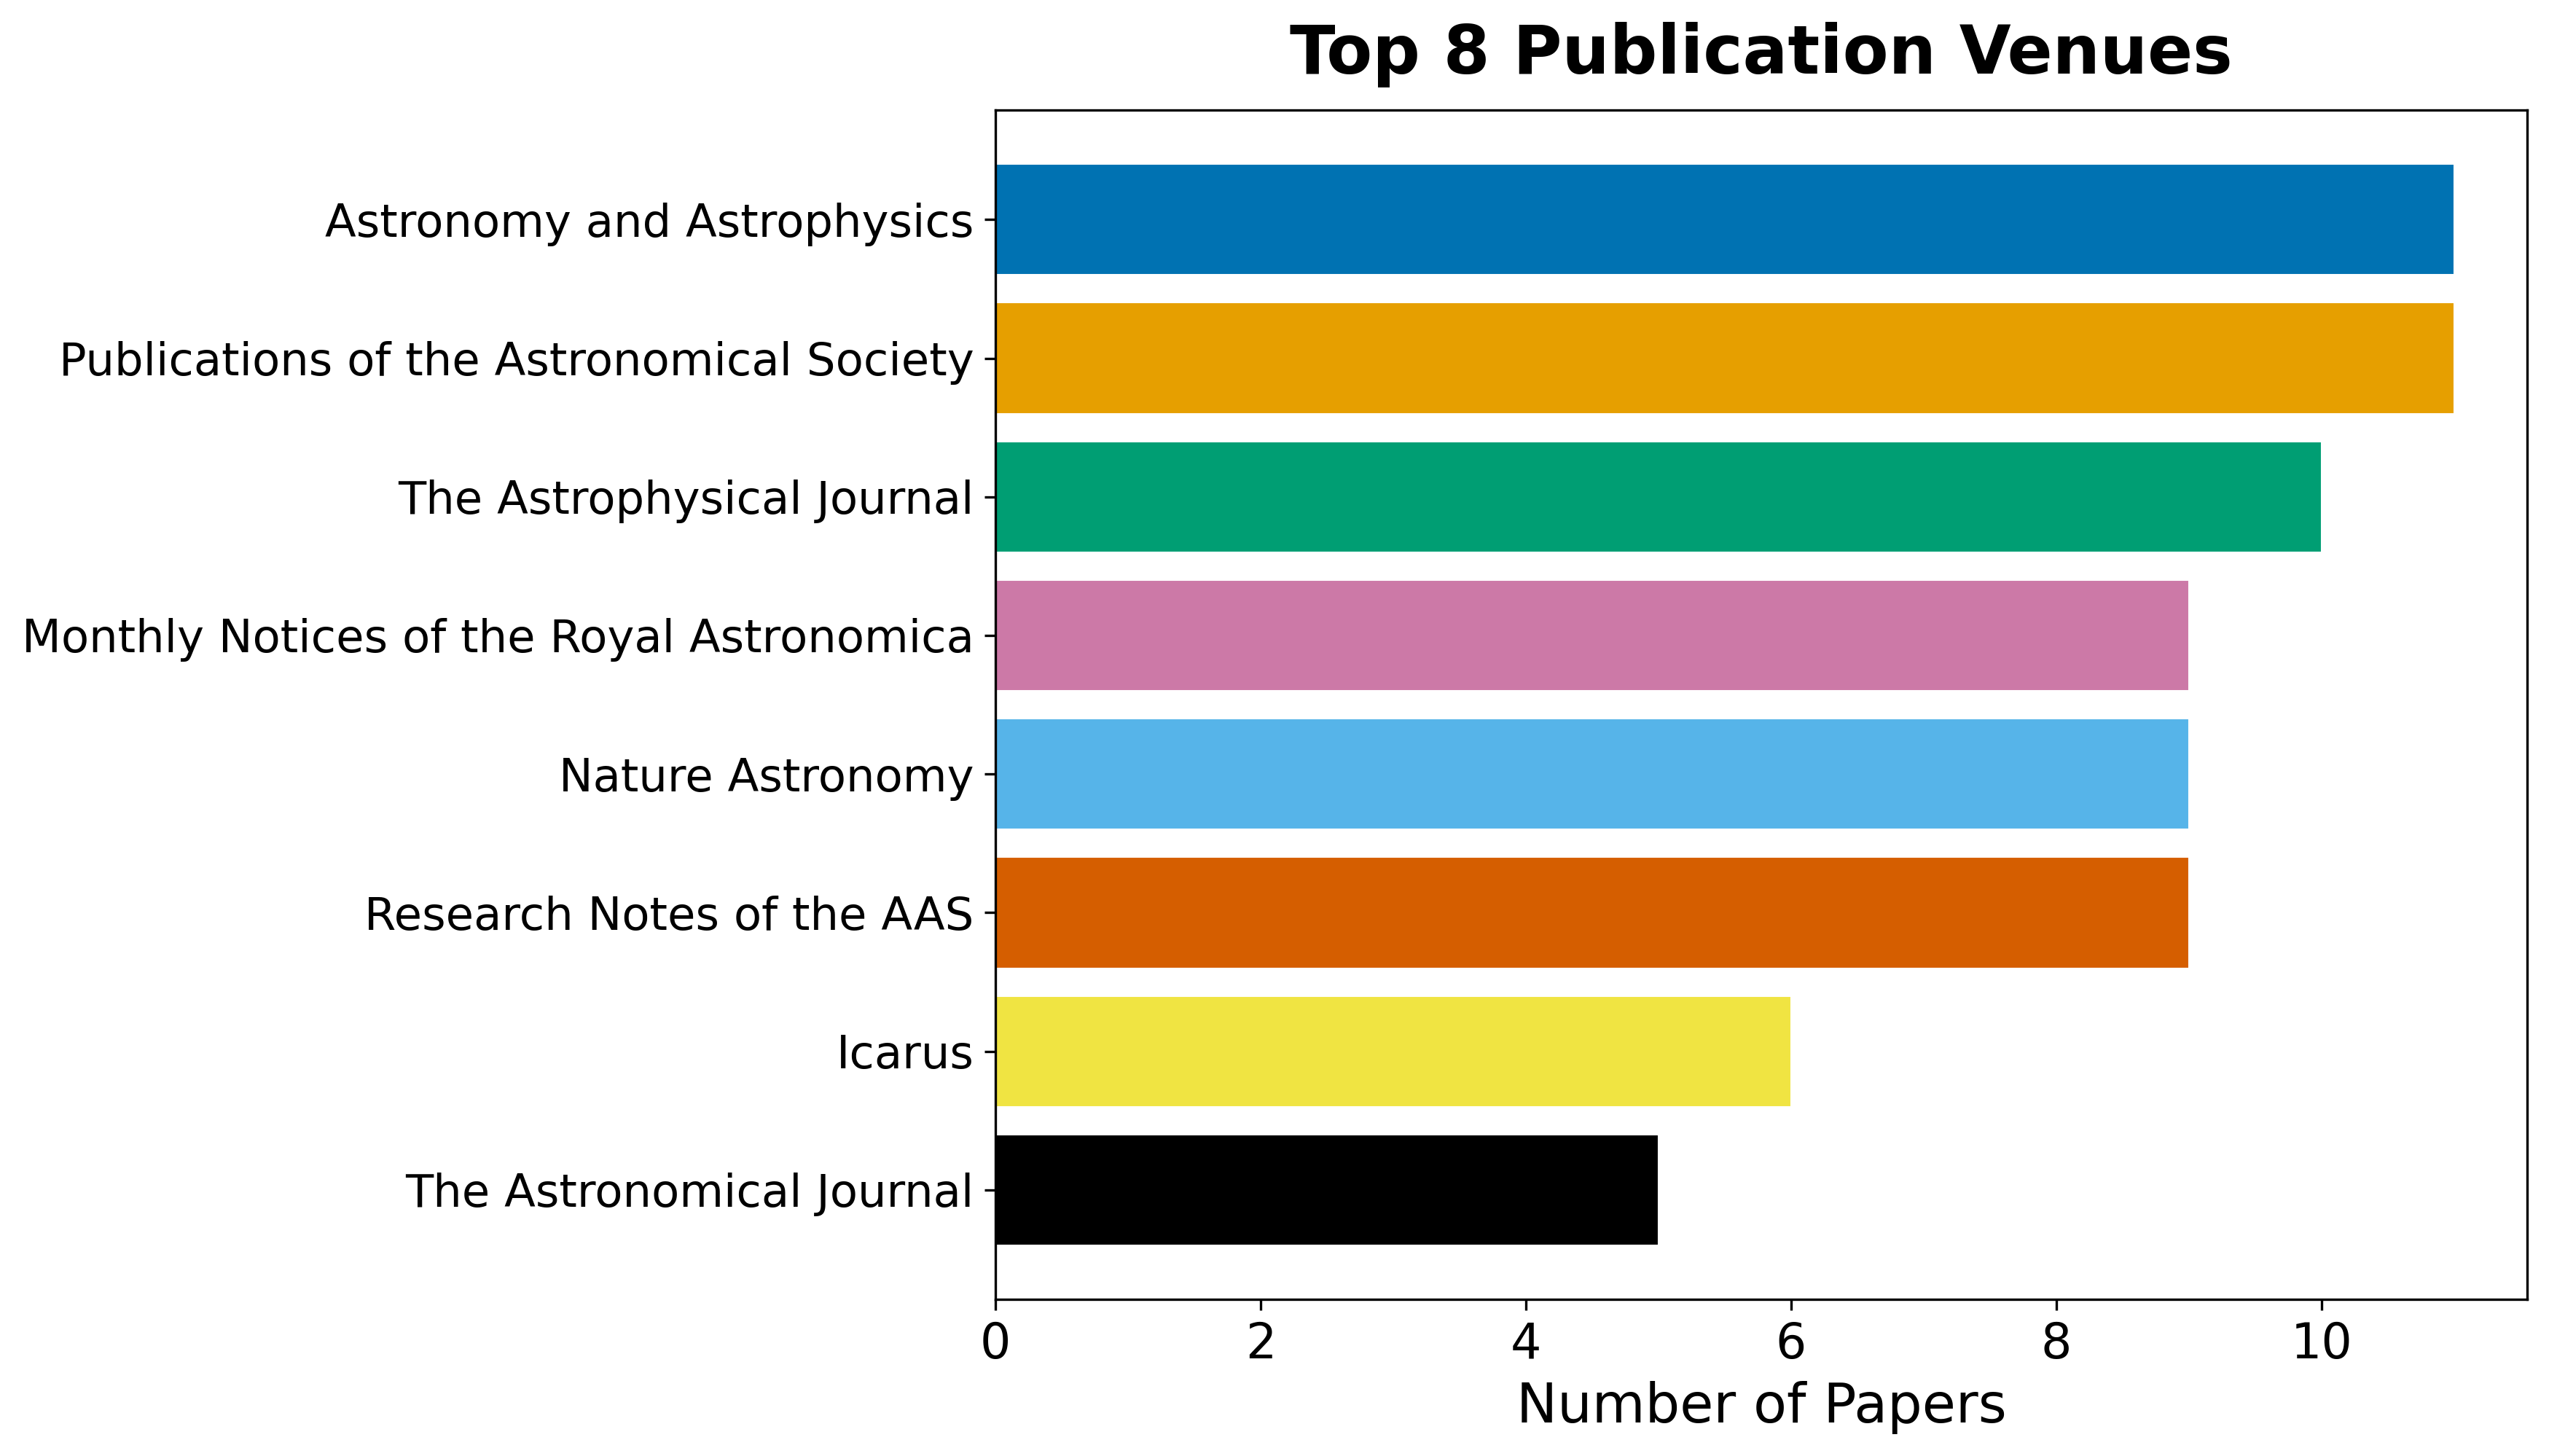
\includegraphics{../figures/top_venues.png}
\caption{Top publication venues for \{\{SEARCH\_TERM\_TITLE\}\}. The
horizontal bar chart shows the venues with the most retained records; it
describes this corpus rather than the complete
field.}\label{fig:top_venues}
\end{figure}

\textbf{Table 5. Top authors by publication count.}

\{\{TOP\_AUTHORS\_TABLE\}\}

\begin{figure}
\centering
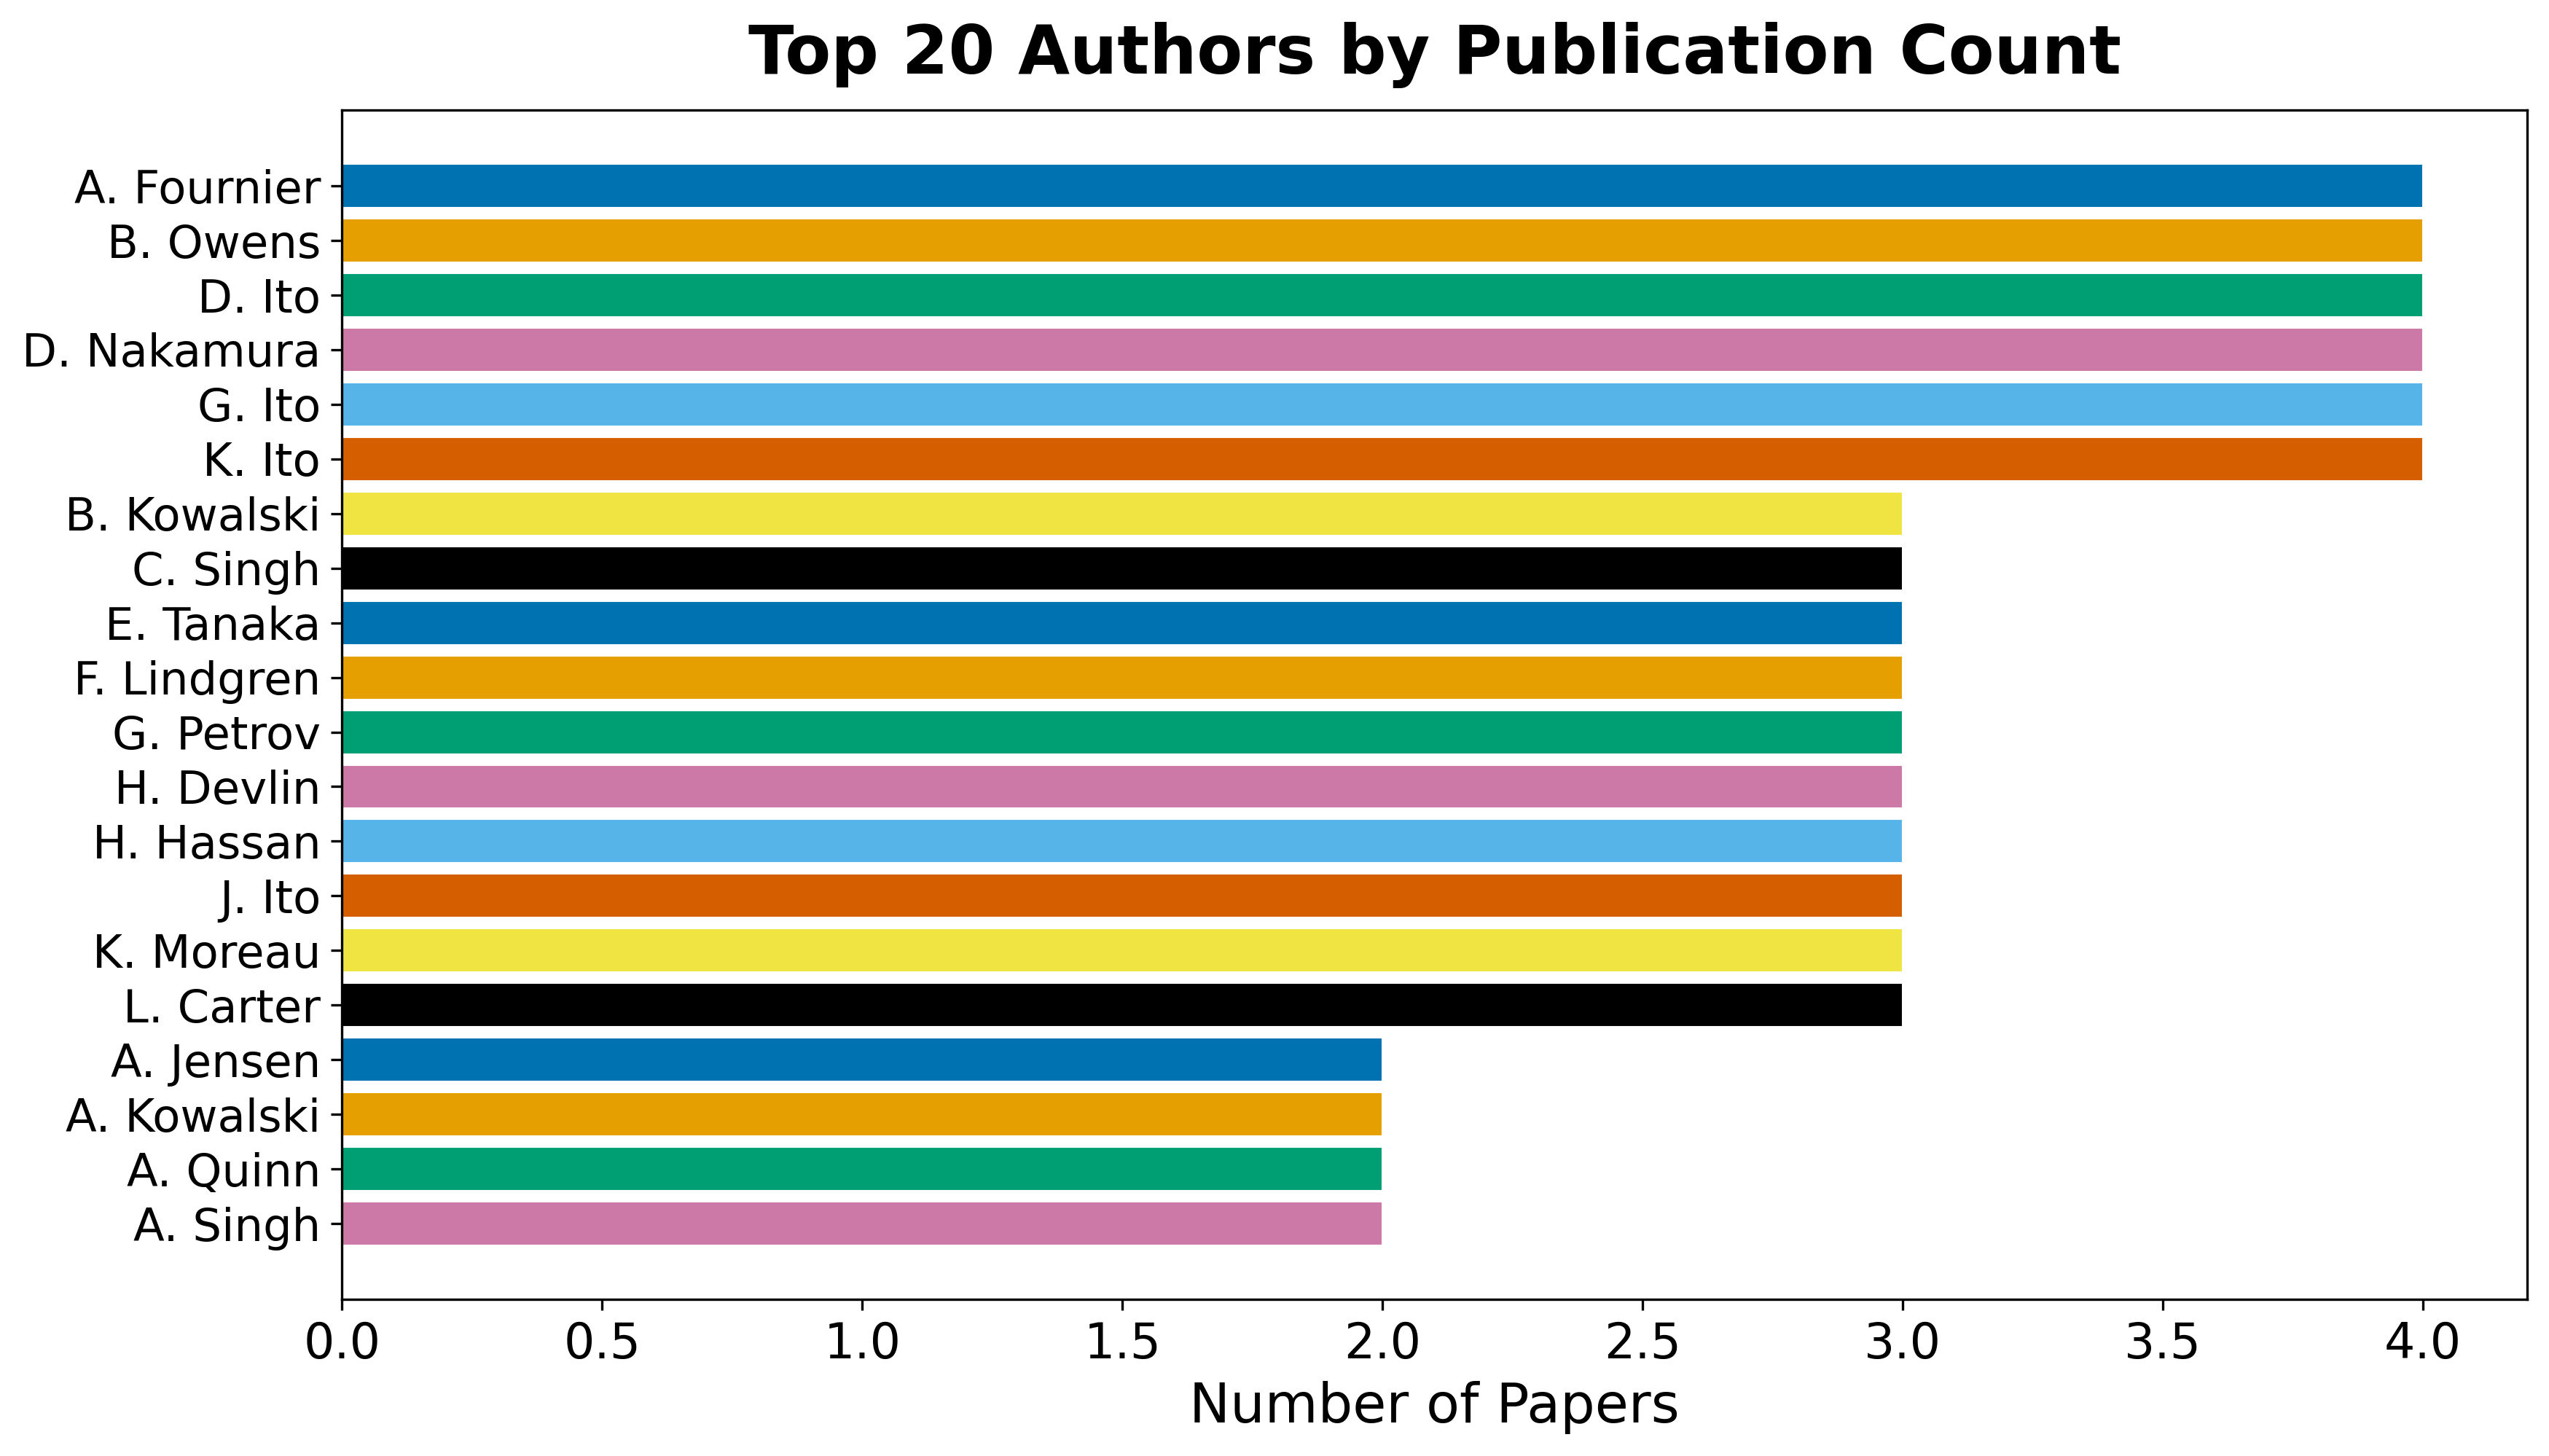
\includegraphics{../figures/author_productivity.png}
\caption{Author productivity for \{\{SEARCH\_TERM\_TITLE\}\}. The
horizontal bar chart shows authors with the most retained records; names
and counts depend on source coverage and
deduplication.}\label{fig:author_productivity}
\end{figure}
\end{frame}

\end{document}
